% Options for packages loaded elsewhere
% Options for packages loaded elsewhere
\PassOptionsToPackage{unicode}{hyperref}
\PassOptionsToPackage{hyphens}{url}
\PassOptionsToPackage{dvipsnames,svgnames,x11names}{xcolor}
%
\documentclass[
  11pt,
  letterpaper,
  DIV=11,
  numbers=noendperiod]{scrartcl}
\usepackage{xcolor}
\usepackage{amsmath,amssymb}
\setcounter{secnumdepth}{-\maxdimen} % remove section numbering
\usepackage{iftex}
\ifPDFTeX
  \usepackage[T1]{fontenc}
  \usepackage[utf8]{inputenc}
  \usepackage{textcomp} % provide euro and other symbols
\else % if luatex or xetex
  \usepackage{unicode-math} % this also loads fontspec
  \defaultfontfeatures{Scale=MatchLowercase}
  \defaultfontfeatures[\rmfamily]{Ligatures=TeX,Scale=1}
\fi
\usepackage{lmodern}
\ifPDFTeX\else
  % xetex/luatex font selection
\fi
% Use upquote if available, for straight quotes in verbatim environments
\IfFileExists{upquote.sty}{\usepackage{upquote}}{}
\IfFileExists{microtype.sty}{% use microtype if available
  \usepackage[]{microtype}
  \UseMicrotypeSet[protrusion]{basicmath} % disable protrusion for tt fonts
}{}
\makeatletter
\@ifundefined{KOMAClassName}{% if non-KOMA class
  \IfFileExists{parskip.sty}{%
    \usepackage{parskip}
  }{% else
    \setlength{\parindent}{0pt}
    \setlength{\parskip}{6pt plus 2pt minus 1pt}}
}{% if KOMA class
  \KOMAoptions{parskip=half}}
\makeatother
% Make \paragraph and \subparagraph free-standing
\makeatletter
\ifx\paragraph\undefined\else
  \let\oldparagraph\paragraph
  \renewcommand{\paragraph}{
    \@ifstar
      \xxxParagraphStar
      \xxxParagraphNoStar
  }
  \newcommand{\xxxParagraphStar}[1]{\oldparagraph*{#1}\mbox{}}
  \newcommand{\xxxParagraphNoStar}[1]{\oldparagraph{#1}\mbox{}}
\fi
\ifx\subparagraph\undefined\else
  \let\oldsubparagraph\subparagraph
  \renewcommand{\subparagraph}{
    \@ifstar
      \xxxSubParagraphStar
      \xxxSubParagraphNoStar
  }
  \newcommand{\xxxSubParagraphStar}[1]{\oldsubparagraph*{#1}\mbox{}}
  \newcommand{\xxxSubParagraphNoStar}[1]{\oldsubparagraph{#1}\mbox{}}
\fi
\makeatother

\usepackage{color}
\usepackage{fancyvrb}
\newcommand{\VerbBar}{|}
\newcommand{\VERB}{\Verb[commandchars=\\\{\}]}
\DefineVerbatimEnvironment{Highlighting}{Verbatim}{commandchars=\\\{\}}
% Add ',fontsize=\small' for more characters per line
\usepackage{framed}
\definecolor{shadecolor}{RGB}{241,243,245}
\newenvironment{Shaded}{\begin{snugshade}}{\end{snugshade}}
\newcommand{\AlertTok}[1]{\textcolor[rgb]{0.68,0.00,0.00}{#1}}
\newcommand{\AnnotationTok}[1]{\textcolor[rgb]{0.37,0.37,0.37}{#1}}
\newcommand{\AttributeTok}[1]{\textcolor[rgb]{0.40,0.45,0.13}{#1}}
\newcommand{\BaseNTok}[1]{\textcolor[rgb]{0.68,0.00,0.00}{#1}}
\newcommand{\BuiltInTok}[1]{\textcolor[rgb]{0.00,0.23,0.31}{#1}}
\newcommand{\CharTok}[1]{\textcolor[rgb]{0.13,0.47,0.30}{#1}}
\newcommand{\CommentTok}[1]{\textcolor[rgb]{0.37,0.37,0.37}{#1}}
\newcommand{\CommentVarTok}[1]{\textcolor[rgb]{0.37,0.37,0.37}{\textit{#1}}}
\newcommand{\ConstantTok}[1]{\textcolor[rgb]{0.56,0.35,0.01}{#1}}
\newcommand{\ControlFlowTok}[1]{\textcolor[rgb]{0.00,0.23,0.31}{\textbf{#1}}}
\newcommand{\DataTypeTok}[1]{\textcolor[rgb]{0.68,0.00,0.00}{#1}}
\newcommand{\DecValTok}[1]{\textcolor[rgb]{0.68,0.00,0.00}{#1}}
\newcommand{\DocumentationTok}[1]{\textcolor[rgb]{0.37,0.37,0.37}{\textit{#1}}}
\newcommand{\ErrorTok}[1]{\textcolor[rgb]{0.68,0.00,0.00}{#1}}
\newcommand{\ExtensionTok}[1]{\textcolor[rgb]{0.00,0.23,0.31}{#1}}
\newcommand{\FloatTok}[1]{\textcolor[rgb]{0.68,0.00,0.00}{#1}}
\newcommand{\FunctionTok}[1]{\textcolor[rgb]{0.28,0.35,0.67}{#1}}
\newcommand{\ImportTok}[1]{\textcolor[rgb]{0.00,0.46,0.62}{#1}}
\newcommand{\InformationTok}[1]{\textcolor[rgb]{0.37,0.37,0.37}{#1}}
\newcommand{\KeywordTok}[1]{\textcolor[rgb]{0.00,0.23,0.31}{\textbf{#1}}}
\newcommand{\NormalTok}[1]{\textcolor[rgb]{0.00,0.23,0.31}{#1}}
\newcommand{\OperatorTok}[1]{\textcolor[rgb]{0.37,0.37,0.37}{#1}}
\newcommand{\OtherTok}[1]{\textcolor[rgb]{0.00,0.23,0.31}{#1}}
\newcommand{\PreprocessorTok}[1]{\textcolor[rgb]{0.68,0.00,0.00}{#1}}
\newcommand{\RegionMarkerTok}[1]{\textcolor[rgb]{0.00,0.23,0.31}{#1}}
\newcommand{\SpecialCharTok}[1]{\textcolor[rgb]{0.37,0.37,0.37}{#1}}
\newcommand{\SpecialStringTok}[1]{\textcolor[rgb]{0.13,0.47,0.30}{#1}}
\newcommand{\StringTok}[1]{\textcolor[rgb]{0.13,0.47,0.30}{#1}}
\newcommand{\VariableTok}[1]{\textcolor[rgb]{0.07,0.07,0.07}{#1}}
\newcommand{\VerbatimStringTok}[1]{\textcolor[rgb]{0.13,0.47,0.30}{#1}}
\newcommand{\WarningTok}[1]{\textcolor[rgb]{0.37,0.37,0.37}{\textit{#1}}}

\usepackage{longtable,booktabs,array}
\usepackage{calc} % for calculating minipage widths
% Correct order of tables after \paragraph or \subparagraph
\usepackage{etoolbox}
\makeatletter
\patchcmd\longtable{\par}{\if@noskipsec\mbox{}\fi\par}{}{}
\makeatother
% Allow footnotes in longtable head/foot
\IfFileExists{footnotehyper.sty}{\usepackage{footnotehyper}}{\usepackage{footnote}}
\makesavenoteenv{longtable}
\usepackage{graphicx}
\makeatletter
\newsavebox\pandoc@box
\newcommand*\pandocbounded[1]{% scales image to fit in text height/width
  \sbox\pandoc@box{#1}%
  \Gscale@div\@tempa{\textheight}{\dimexpr\ht\pandoc@box+\dp\pandoc@box\relax}%
  \Gscale@div\@tempb{\linewidth}{\wd\pandoc@box}%
  \ifdim\@tempb\p@<\@tempa\p@\let\@tempa\@tempb\fi% select the smaller of both
  \ifdim\@tempa\p@<\p@\scalebox{\@tempa}{\usebox\pandoc@box}%
  \else\usebox{\pandoc@box}%
  \fi%
}
% Set default figure placement to htbp
\def\fps@figure{htbp}
\makeatother





\setlength{\emergencystretch}{3em} % prevent overfull lines

\providecommand{\tightlist}{%
  \setlength{\itemsep}{0pt}\setlength{\parskip}{0pt}}



 


\KOMAoption{captions}{tableheading}
\makeatletter
\@ifpackageloaded{caption}{}{\usepackage{caption}}
\AtBeginDocument{%
\ifdefined\contentsname
  \renewcommand*\contentsname{Table of contents}
\else
  \newcommand\contentsname{Table of contents}
\fi
\ifdefined\listfigurename
  \renewcommand*\listfigurename{List of Figures}
\else
  \newcommand\listfigurename{List of Figures}
\fi
\ifdefined\listtablename
  \renewcommand*\listtablename{List of Tables}
\else
  \newcommand\listtablename{List of Tables}
\fi
\ifdefined\figurename
  \renewcommand*\figurename{Figure}
\else
  \newcommand\figurename{Figure}
\fi
\ifdefined\tablename
  \renewcommand*\tablename{Table}
\else
  \newcommand\tablename{Table}
\fi
}
\@ifpackageloaded{float}{}{\usepackage{float}}
\floatstyle{ruled}
\@ifundefined{c@chapter}{\newfloat{codelisting}{h}{lop}}{\newfloat{codelisting}{h}{lop}[chapter]}
\floatname{codelisting}{Listing}
\newcommand*\listoflistings{\listof{codelisting}{List of Listings}}
\makeatother
\makeatletter
\makeatother
\makeatletter
\@ifpackageloaded{caption}{}{\usepackage{caption}}
\@ifpackageloaded{subcaption}{}{\usepackage{subcaption}}
\makeatother
\usepackage{bookmark}
\IfFileExists{xurl.sty}{\usepackage{xurl}}{} % add URL line breaks if available
\urlstyle{same}
\hypersetup{
  pdftitle={Research Paper --- Advanced Analytics in Sports},
  pdfauthor={Ava Mizrahi},
  colorlinks=true,
  linkcolor={blue},
  filecolor={Maroon},
  citecolor={Blue},
  urlcolor={Blue},
  pdfcreator={LaTeX via pandoc}}


\title{Research Paper --- Advanced Analytics in Sports}
\author{Ava Mizrahi}
\date{}
\begin{document}
\maketitle


In modern sports analytics, many of the traditional statistics used do
not provide a full understanding of performance of players and teams.
Soccer is a low scoring game, so this problem is especially heightened
since outcomes can be highly influenced by randomness instead of skill.
Because of this, analysts created a metric called expected goals (xG)
that provides each shot with a probability of resulting in a goal that
is based on different factors such as angle, distance from the goal,
body part used to make the shot, and defensive pressure. xG is a great
metric, but it isn't without its faults.

This article, ``Separating Chance Quality and Player Ability in xG,''
written by Alex Felices, focuses on how the xG metric can be improved
when analyzing soccer players and teams. The main thesis is that
traditional xG models do not distinguish between the quality of a
scoring opportunity and the skill of the player taking the shot. This
can lead to a misinterpretation of a player or team's skill. The article
aims to determine whether players who consistently exceed their xG are
truly better finishers or whether existing models are missing important
contextual factors.

To address this concern, the article reviews a study that developed its
own xG model using event stream data, which is data that contains a
sequential track of every move on the ball during a match such as
passes, shots, fouls, dribbles, etc. along with additional contextual
measures. Felices begins with an explanation of how crucial the xG
metric has become to performance analysis, recruitment, and betting with
soccer. The author wants to create a new xG model that is more reliable
for predicting the likelihood of a shot being a goal and make it similar
to industry models.

The model focuses only on open play shots, which are shots that are
taken during live gameplay rather than from a corner kick, free kick, or
penalty. The model uses a dataset of over 15,000 shots from La Liga.
Initially, 95 variables were considered, which were later reduced to a
smaller set of important features, including spatial data, contextual
information (such as defender and goalkeeper positioning), and shot
characteristics. The model began with a logistic regression baseline,
which performed poorly by underpredicting high quality chances of a
goal. After adding more variables, the model's accuracy was greatly
improved. The final model using machine learning along with additional
variables enhanced performance and gave results that matched closely
with real world outcomes.

The author then introduces position adjusted and player adjusted xG
models. After analyzing forwards, midfielders, and defenders, it was
found that forwards were the most efficient finishers compared to
midfielders and defenders and this increased xG. This model proves that
the ability to finish varies significantly by position. Next, Lionel
Messi was used as a case study for the player adjusted model since he
tends to exceed his predicted goals. When the Messi adjusted model was
applied to all players, the total xG increased significantly. This means
that individual players have a measurable difference in finishing
ability and it can vary significantly by player.

By determining that both individual player and position can impact xG,
the author concludes that the traditional xG metric is limited since it
does not account for player skill or position and having that additional
context improves accuracy. This adjusted xG model allows for a more
accurate prediction of performance. The key metric in this article is xG
(expected goals), along with the article's addition of the player and
position adjusted xG models. Expected goals is a statistic that assigns
each shot a value between 0 and 1, where 0 means the shot had almost no
chance of becoming a goal and 1 would mean the shot was almost certain
to become a goal. For example, a shot from far outside the box might
have an xG of 0.03, which means shots like that are scored about 3\% of
the time, while a closer shot right in front of an open goal might have
an xG of 0.80.

The first step of calculating xG is to build a dataset of past shots
where each row in the dataset represents one shot, and the response
variable shows whether the shot became a goal (0 for no goal, 1 for a
goal). The dataset also includes predictors that describe the shot. In
the model used in the article, these variables are factors such as the
distance from goal, the angle to goal, the body part used, goalkeeper
position, defender pressure, and other contextual aspects.

After the dataset is built, most of the time, a logistic regression
model is used to fit a probability of scoring since the outcome is
binary (0 or 1). The logistic regression model is

\[
P(\text{goal}) = \frac{1}{1 + e^{-(\beta_0 + \beta_1 x_1 + \beta_2 x_2 + \cdots + \beta_n x_n)}}
\]

where each \(x_i\) represents an attribute of the shot (distance, angle,
etc.) and each \(\beta_i\) is a coefficient estimated from the data.

The total expected goals is calculated as:

\[
\text{Total xG} = \sum_{i=1}^{n} xG_i
\] For example, if a shot has its corresponding values plugged into the
model and gives an output of \(P(\text{goal}) = 0.11\), this means the
shot has an 11\% chance of being scored based on historic shots with
similar statistics.

This article improves this model by adding more detailed contextual
features since the basic model may miss important details. Also, the
player and position adjusted xG models were created to expand further.
The model in the article is no longer a basic xG model that only
estimates the probability that an average player would score the shot.
It now can estimate the probability that a specific player with a
certain position will score.

\begin{Shaded}
\begin{Highlighting}[]
\CommentTok{\# Import dataset}
\ImportTok{import}\NormalTok{ pandas }\ImportTok{as}\NormalTok{ pd}

\NormalTok{shot\_data }\OperatorTok{=}\NormalTok{ pd.read\_csv(}\StringTok{"soccer\_shots\_distance.csv"}\NormalTok{)}
\NormalTok{shot\_data.head()}
\end{Highlighting}
\end{Shaded}

\begin{longtable}[]{@{}lllllllll@{}}
\toprule\noalign{}
& match\_id & shot\_outcome & shot\_type & shot\_body\_part & distance &
competition\_name & season\_name & source\_file \\
\midrule\noalign{}
\endhead
\bottomrule\noalign{}
\endlastfoot
0 & 18242 & Off T & Open Play & Right Foot & 20.000000 & Champions
League & 2014/2015 & Champions\_League\_2014-2015\_shots.csv \\
1 & 18242 & Wayward & Open Play & Head & 12.369317 & Champions League &
2014/2015 & Champions\_League\_2014-2015\_shots.csv \\
2 & 18242 & Goal & Open Play & Left Foot & 8.246211 & Champions League &
2014/2015 & Champions\_League\_2014-2015\_shots.csv \\
3 & 18242 & Off T & Open Play & Right Foot & 22.472205 & Champions
League & 2014/2015 & Champions\_League\_2014-2015\_shots.csv \\
4 & 18242 & Off T & Open Play & Right Foot & 19.313208 & Champions
League & 2014/2015 & Champions\_League\_2014-2015\_shots.csv \\
\end{longtable}

\begin{Shaded}
\begin{Highlighting}[]
\CommentTok{\# Create the goal binary variable }
\NormalTok{shot\_data[}\StringTok{"goal"}\NormalTok{] }\OperatorTok{=}\NormalTok{ (shot\_data[}\StringTok{"shot\_outcome"}\NormalTok{] }\OperatorTok{==} \StringTok{"Goal"}\NormalTok{).astype(}\BuiltInTok{int}\NormalTok{)}

\CommentTok{\# Clean the data}
\NormalTok{shot\_data }\OperatorTok{=}\NormalTok{ shot\_data[[}\StringTok{"goal"}\NormalTok{, }\StringTok{"distance"}\NormalTok{, }\StringTok{"shot\_body\_part"}\NormalTok{, }\StringTok{"shot\_type"}\NormalTok{]].dropna()}

\CommentTok{\# Use only open play shots like the article }
\NormalTok{shot\_data }\OperatorTok{=}\NormalTok{ shot\_data[shot\_data[}\StringTok{"shot\_type"}\NormalTok{] }\OperatorTok{==} \StringTok{"Open Play"}\NormalTok{]}
\end{Highlighting}
\end{Shaded}

\begin{Shaded}
\begin{Highlighting}[]
\ImportTok{import}\NormalTok{ statsmodels.formula.api }\ImportTok{as}\NormalTok{ smf}

\NormalTok{model }\OperatorTok{=}\NormalTok{ smf.logit(}\StringTok{"goal \textasciitilde{} distance + C(shot\_body\_part) + C(shot\_type)"}\NormalTok{, data}\OperatorTok{=}\NormalTok{shot\_data).fit()}

\NormalTok{shot\_data[}\StringTok{"xG"}\NormalTok{] }\OperatorTok{=}\NormalTok{ model.predict(shot\_data)}

\NormalTok{summary }\OperatorTok{=}\NormalTok{ pd.DataFrame(\{}
  \StringTok{"Actual Goals"}\NormalTok{: [shot\_data[}\StringTok{"goal"}\NormalTok{].}\BuiltInTok{sum}\NormalTok{()],}
  \StringTok{"Expected Goals"}\NormalTok{: [shot\_data[}\StringTok{"xG"}\NormalTok{].}\BuiltInTok{sum}\NormalTok{()]}
\NormalTok{\})}

\BuiltInTok{print}\NormalTok{(summary)}

\CommentTok{\# The total expected goals closely matches the total observed goals because the model was trained and used on the same dataset.}
\end{Highlighting}
\end{Shaded}

\begin{verbatim}
Optimization terminated successfully.
         Current function value: 0.293346
         Iterations 7
   Actual Goals  Expected Goals
0          1439          1439.0
\end{verbatim}

\begin{Shaded}
\begin{Highlighting}[]
\ImportTok{import}\NormalTok{ matplotlib.pyplot }\ImportTok{as}\NormalTok{ plt}
\NormalTok{plt.scatter(shot\_data[}\StringTok{"distance"}\NormalTok{], shot\_data[}\StringTok{"xG"}\NormalTok{], alpha}\OperatorTok{=}\FloatTok{0.2}\NormalTok{)}
\NormalTok{plt.xlabel(}\StringTok{"Shot Distance"}\NormalTok{)}
\NormalTok{plt.ylabel(}\StringTok{"xG"}\NormalTok{)}
\NormalTok{plt.title(}\StringTok{"Expected Goals vs Shot Distance"}\NormalTok{)}
\NormalTok{plt.show()}
\end{Highlighting}
\end{Shaded}

\pandocbounded{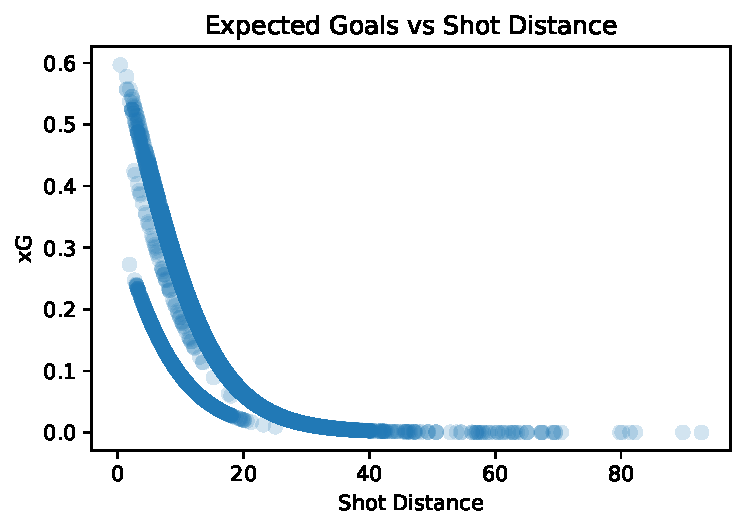
\includegraphics[keepaspectratio]{submission-research-paper-final_files/figure-pdf/cell-5-output-1.pdf}}

One of the main strengths of the xG metric is that it is a more accurate
measure of performance instead of just shooting percentage. It does take
into account that goals are not the only thing that can determine the
quality of a player or team. A player could score a lot of goals, but
only take the easiest shots. The xG model in general measures the
likelihood of a shot becoming a goal, which helps to separate luck from
skill. Since soccer is such a low scoring sport, outcomes can be heavily
impacted by randomness. With the xG model, analysts can see if a player
is over or under performing based on the quality of their chances at a
goal, which is helpful for predicting future success because players who
are constantly getting high xG are more likely to continue scoring in
the future.

In the article, the xG used is an improvement from traditional xG
metrics because it adds more contextual variables for higher accuracy.
The model from the article adds variables such as defensive pressure and
goalkeeper position. With more variables included, the article's xG
model is able to better simulate real world games and situations. The
article also looks at player and position adjusted xG metrics. These
adjustments account for differing players and positions rather than
assuming everything is the same.

Even though the xG metric has improved significantly, it still has its
limitations. One negative feature about this metric is that a high
quality and complete dataset is needed in order to use it. It can be
difficult to capture every variable that can influence a shot, even with
the additional variables, so some outcomes can still be inaccurate.
Also, the article mentions using more complex machine learning methods
to improve the model. This would be good for accuracy, but can make it
more difficult to understand exactly how each variable individually
impacts the outcome.

Another limitation to the xG metric is that finishing ability is
inconsistent and can be difficult to measure in some circumstances. In
the real world, players can go through periods of underperforming or
overperforming due to external factors which can make it difficult to
determine if a player's performance truly depends on skill or
randomness. The model could overestimate differences in finishing
ability and blame outcomes on lack of skill when it really could be
randomness.

The improved xG metric directly supports the author's main argument by
showing that traditional xG models may not fully represent player skill
level. The author's thesis is that the traditional xG metric combines
skill and chance, which can lead to incorrect conclusions. From
introducing more variables and position and player adjustments, the new
metric separates skill and chance and proves that the player and
position differences make an impact on the outcome. From the example in
the article, forwards tend to outperform xG and Lionel Messi also
consistently exceeds his xG over time. This supports the claim that some
players are just better finishers on average rather than just having
better chances at scoring.

There are still some concerns with using the xG metric to support the
argument because the player adjusted model mostly relies on historical
data and can be incorrect if the player is on a bad playing streak or
just does not have a good amount of data. The model also consistently
assumes that the differences between actual and expected goals is solely
due to player skill level. This is not always true because there could
still be some variation caused by randomness. Due to these limitations,
the improved xG metric does not fully prove that luck and skill can
completely be separated when determining scoring ability.

The article mentions using machine learning methods and logistic
regression to improve the xG model. Logistic regression is the main
method used for predictions. Using a logistic regression model is
appropriate because it allows the outcome to be binary (Goal = 1, No
Goal = 0) and is easy to interpret probabilities. The article then takes
the model to the next level by appropriately incorporating machine
learning methods for improvements. Using machine learning methods shows
the limitations of a basic model and the benefits of a more advanced
model. There are no other main metrics mentioned other than the xG
model, which is the main focus of the article.

Overall, the article shows that even though expected goals (xG) is a
beneficial metric for determining player skill level in soccer, there
are still some limitations to it that need to be considered during
analysis. The author found from looking at players and positions
individually, the traditional xG metric can misinterpret skill level and
treat players as if they all have the same finishing ability. After
using higher level methods to make an improved model, the analysis
recognizes that no model can fully capture every aspect of the game and
make a completely accurate prediction. However, the xG metric is a more
complete and detailed way of analyzing player performance and is a
valuable tool in soccer analytics.\\
```




\end{document}
